\makeatletter
\def\input@path{{../../}}
\makeatother
\documentclass[../../main.tex]{subfiles}

\graphicspath{
	{../../img/}
	{../img/}
	{img/}
}

\begin{document}
	
	\begin{thm}[о сведении вычисления 3И к 2И]
		Пусть $ H $~--- цилиндроид вдоль оси $ Oz $, т.~е. 
		\begin{equation}
		\label{lec14:1}
		H = \left\lbrace \left( x, y, z \right) \in \R^3\ |
		\ \left( x, y \right) \in D \subset \R^2;\ p \leq z \leq q \right\rbrace
		\end{equation}
		где $ p, q \in \R $, а $ D $~--- квадрируемая область в $ \R^2 $.
		Если $f \in C(H)$, то в случае, когда $H$~--- компакт 
		в $\R^3$, \eqref {lec_13, num_23} записывается в виде
		\begin{equation}
		\label{lec14:2}
		I = \iint\limits_D \left( \int\limits_p^q 
		f \left( x, y, z \right) dz \right) dx dy.
		\end{equation}
	\end{thm}

		
	\begin{proof}
		Доказательство проводится по той же схеме, что и при вычислении 2И по 
		прямоугольнику. В начале рассмотрим произвольное разбиение $P_0 = \left\{ 
		z_k \right\}$, $k = 
		\overline{0, m}$ отрезка $\left[p, q\right]$, $p = z_0 < z_1 < \ldots < z_{m 
		- 1} < z_m = q.$ Далее в силу непрерывности $f$ на $H$ имеем:
		
		\begin{equation}
		\exists F\left(x, y\right) = \int\limits_{p}^{q} f\left(x, y, z\right) dz.
		\label{lec14:3}
		\end{equation}\\
		Далее, проведя произвольное разбиение $\widetilde{P_0}$ квадрируемого 
		компакта $D \subset 
		\R^2$, являющегося проекцией $H \subset \R^3$ на $Oxy$, получим
		$\widetilde{P_0} = \left\{D_j \right\},\ j = \overline{1, l}, \text{ где } 
		\bigcup\limits_{j = 1}^l D_j = D$ и $\mes(D_i \cap D_j) = 0,\ \forall i \neq 
		j$, т.~е. квадрируемые части разбиения $\widetilde{P_0}$ между собой могут 
		иметь общими 
		лишь, может быть, граничные точки.
		
		Выбирая произвольным образом множество отмеченных точек $\widetilde{Q_0} = 
		\left\{ M_j \right\},\ M_j = \left(x_j, y_j\right) \in D,\ j = \overline{1, 
		l}$, в соответствии с \eqref{lec14:3} рассмотрим интеграл Римана
		\begin{equation} 
		I_{kj} = \int\limits_{z_{k-1}}^{z_k} f(x_j, y_j, z)dz = F_k (M_j),\; j = 
		\overline{1, l},  \label{lec14:4}
		\end{equation}
		
		где \[F_k(x, y) = \int\limits_{z_k - 1}^{z_k} f\left(x, y, z\right)dz,\ k = 
		\overline{1, m}.\]
		 
		По теореме о среднем для ОИ
		\begin{equation}
			\exists t_{kj} \in \left[z_{k - 1}, z_k 
		\right],\ k = \overline{1, m} \text{ такие, что }
		 	I_{kj} = f(x_j, y_j, t_{kj})\left(z_k - z_{k - 1}\right) = 
		 	F(N_{kj}) \Delta z_k, \label{lec14:5}
		 \end{equation}
		где \[\begin{cases}
		N_{kj} = (x_j, y_j, t_{kj}) = (M_j, t_{kj}),\\
		\Delta z_k = z_k - z_{k - 1}, \\ k = \overline{1, m},\ j = \overline{1, l}.
		\end{cases}\]
		
		Отсюда при $\widetilde{d_0} = \diam \widetilde{P_0} \to 0$ имеем: 
		
		\begin{equation}
		\iint\limits_D F\left(x, y\right) dxdy = \lim\limits_{\widetilde{d_0} 
		\to 0} \widetilde{\sigma_0}, \label{lec14:6}
		\end{equation}
		где 
		\begin{equation}
		\begin{gathered}
		\widetilde{\sigma_0} = \sum\limits_{j = 1}^{l} F\left(M_j\right) \Delta 
		D_j = \left(\int\limits_{z_0 = p}^{z_1} + \ldots + \int\limits_{z_m - 
		1}^{z_m = q} \right)\D D_j = \sum\limits_{j = 1}^{l} \sum\limits_{k = 1}^{m} 
		\left(\int\limits_{z_k - 1}^{z_k} f(M_j, z)dz\right) \Delta D_j = \\ 
		= \sum\limits_{j = 1}^{l} \sum\limits_{k = 1}^{m} I_{kj} \Delta D_j = 
		\sum\limits_{j = 1}^{l} \sum\limits_{k = 1}^{m} f\left(N_{kj}\right) \Delta 
		z_k \Delta D_j, \label{lec14:7}
		\end{gathered}
		\end{equation}
		где $\Delta D_j = \mes D_j$~--- площадь $D_j$.
		
		\eqref{lec14:7} является специальной интегральной суммой $\sigma_0$ для 
		\eqref{lec14:2}, построенной на разбиении $P = \{ H_k \},\ k = 
		\overline{1, m},$ на множестве специально отмеченных точек $Q = \left\{ 
		N_{kj}\right\}$, где 
		\[
		\begin{cases}
		H_{kj} = D_j \times \left[z_{k - 1}, z_k\right],\\
		N_{kj} = (x_j, y_j, t_{kj}) \in H_{kj}, \\
		k = \overline{1, m}, \ j = \overline{1, l}.
		\end{cases} 
		\]
		
		Из непрерывности исходной функции предел этих специальных интегральных сумм 
		рассмотренного 3И будет такой же, что и у общей интегральной суммы, поэтому 
		при $d = \diam P \to 0$ получаем $0 \leq \diam \widetilde{P} < d \implies d 
		\to 0$ для рассматриваемого кубируемого компакта $H \subset \R^3$ следует
		\begin{equation}
		I = \lim\limits_{d \to 0} \sigma_0 = \iint\limits_D  F\left(x, y\right) dxdy 
		= 
		\iint\limits_D \left(\int\limits_{p}^{q} f(x, y,z) dz\right) 
		dxdy, \label{lec14:9}
		\end{equation}
		что и требовалось доказать.
	\end{proof}
	
	\begin{rems}
		\quad
		\begin{enumerate}
			\item По аналогии с 2И, \eqref{lec14:9} на практике записывается в виде 
			повторных 
			интегралов:
			\begin{equation}
			\iiint\limits_{H} f \left( x, y, z \right) dx dy dz = \iint\limits_{D} 
			dx dy \int\limits_{p}^{q} f\left(x, y, 
			z\right) dz. \label{lec_14, num_1}
			\end{equation}
			
			\item Если кубируемый компакт $H \subset \R$ является цилиндроидом вдоль 
			оси $Oz$, 
			т.~е. 
			\[H = \left\{\left(x, y, z \right) \in \R^3 \; \vline \; p \left(x, 
			y\right) \leq z \leq q \left(x, y \right);\  \left(x, y\right) \in D,
			\right\} \]
			где $p\left(x, y\right)$ и $q\left(x, y\right)$ непрерывны на квадрируемом 
			компакте $D \subset \R^2$, который является проекцией $H$ на плоскость 
			$Oxy$, то тогда для $f 
			\in C\left(H\right)$, как и для 2И получаем представление
			\[\iiint\limits_{H} f \left( x, y, z \right) dx dy dz = \iint\limits_{D} 
			dx dy \int\limits_{p\left(x, y\right)}^{q\left(x, y \right)} f\left(x, y, 
			z\right) dz.\]
			
			\item Если кубируемый компакт $H \subset \R^3$ является цилиндроидом вдоль 
			оси 
			$Oz$, то в случае \eqref{lec_14, num_1} для квадрируемого компакта $D 
			\subset \R^2$, являющегося криволинейной трапецией вдоль оси $Oy$, т.~е.
			\[D = \left\{\left(x, y\right) \in \R^2 \; \vline \; c \left(x\right) \leq 
			y \leq d \left(x \right),\ a \leq x \leq b \right\}, \]
			где $c(x)$ и $d(x)$ непрерывны на $\left[a, b\right]$, имеем:
			\begin{equation}
			\iiint\limits_{\substack{
				p\left(x, y\right) \leq z \leq q\left(x, y\right)\\
				c\left(x\right) \leq y \leq d\left(x\right)\\
				a \leq x \leq b
				}} f \left( x, y, z \right) dx dy dz = \int\limits_{a}^{b} dx 
				\int\limits_{d\left(x\right)}^{c\left(x\right)} dy \int\limits_{p\left(x, 
				y\right)}^{q\left(x, y\right)} f(x, y, z) dz, \label{lec_14, num_2}
			\end{equation}
			где также предполагается, что $p\left(x, y\right)$ и $q\left(x, y\right)$ 
			непрерывны на $D$.
			Получили представление 3И через соответствующие повторные интегралы.
			
			\item Формула \eqref{lec_14, num_2} естественным образом обобщается на 
			случай соответствующих цилиндроидов и их проекций вдоль других координатных 
			осей (всего получаем $3! = 6$ возможностей). В общем случае, когда 
			кубируемый компакт $H \subset \R^3$ является объединением конечного числа 
			таких цилиндроидов, вычисление 3И сводится к вычислению соответствующих 
			интегралов по элементарным цилиндроидам вдоль каких-либо осей. 
		\end{enumerate}
	\end{rems}

	\begin{example}
		Для непрерывной на $\left[0, 1\right]$ функции $g\left(z \right)$ рассмотрим 
		3И, заданный в виде повторных интегралов:
			\[I_0 = \int\limits_{-1}^1dx\int\limits_{-\sqrt{1 - x^2}}^{\sqrt{1 - 
			x^2}}dy\int\limits_{x^2 + y^2}^1 g\left(z\right)dz.\]
		
		В данном случае имеем
		
		\[I_0 = \iiint\limits_{H} g(z) dxdydz,\]
		где $H$~--- компакт в $\R^3$, ограниченный в пространстве параболлой $z = 
		x^2 + 
		y^2$ и плоскостью $z = 1$, проекцией которой на плоскость $Oxy$ является 
		круг $D: x^2 + y^2 \leq 1$.
		
		\begin{center}
		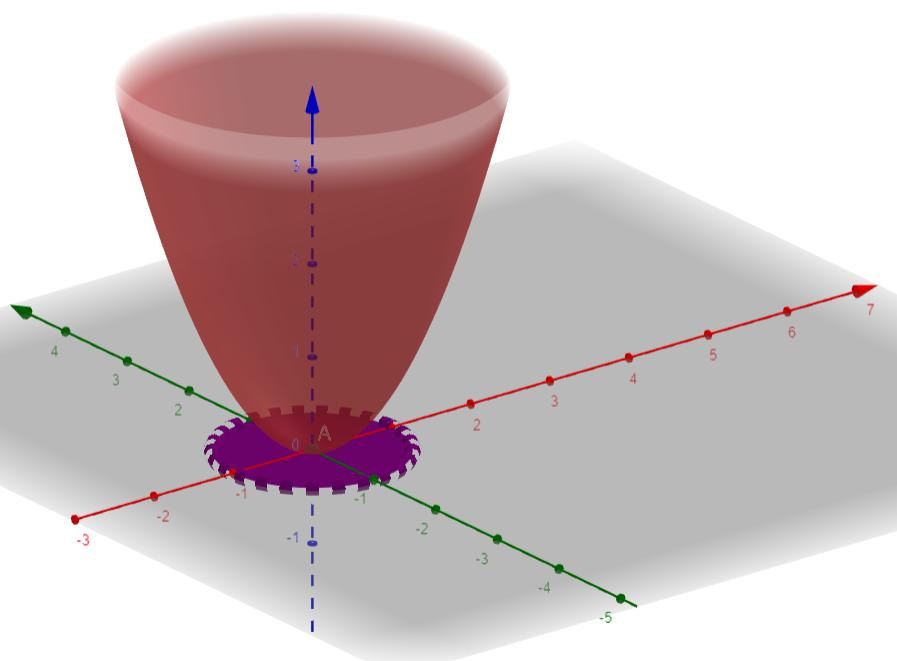
\includegraphics[scale = 0.7]{lec14.jpg}
		\end{center}
		
		Рассматривая $H$ как составную часть цилиндроида вдоль $Oy$, имеем:
		
		\[H = \left\{\left(x, y, z\right) \in \R^3 \ |\ -\sqrt{z - x^2} \leq y 
		\leq \sqrt{z - x^2},\ -\sqrt{z} \leq x \leq \sqrt{z},\ 0 \le z \le 1 
		\right\}.\]
		
		Переходя в таком виде снова к повторным пределам, имеем:
		
		\[
		\begin{gathered}
		I_0 = 
		\int\limits_0^1dz\int\limits_{-\sqrt{z}}^{\sqrt{z}}dx\int\limits_{-\sqrt{z - 
		x^2}}^{\sqrt{z - x^2}}g\left(z\right)dy = 
		2\int\limits_0^1dz\int\limits_{-\sqrt{z}}^{\sqrt{z}}g\left(z\right)\sqrt{z - 
		x^2}dx = \\ =
		\left[\int\sqrt{z - x^2}dx = \frac{x}{2}\sqrt{z - x^2} + 
		\frac{z}{2}\arcsin{\frac{x}{\sqrt{z}}} + C\right] = \\ = 
		4 \int\limits_0^1 g\left(z\right) \left[ \frac{x}{2}\sqrt{z - x^2} + 
		\frac{z}{2}\arcsin{\frac{x}{\sqrt{z}}}\right]_{x=0}^{x=\sqrt{z}}dz= 2 
		\int\limits_0^1 g\left(z\right) \left[x\sqrt{z - x^2} + 
		z\arcsin{\frac{x}{\sqrt{z}}}\right]_{x=0}^{x=\sqrt{z}}dz = \\
		= 2 \int\limits_0^1 g\left(z\right) \left(\sqrt{z} \cdot \sqrt{z-z} + 
		z \cdot \arcsin{\frac{\sqrt{z}}{\sqrt{z}}}\right) dz = 2 \int\limits_0^1 
		g\left(z\right) \cdot z \cdot \frac{\pi}{2} dz = \pi \int\limits_0^1 z \cdot 
		g\left(z\right)dz. 
		\end{gathered}\]
	\end{example}

	\section{Замена переменных в $n$-кратном интеграле}
	
	Рассмотрим множества $D \subset \R^n$ и $G \subset \R^n$. Множество $D$ будем 
	рассматривать в ПДСК\\ $Ox_1 \ldots x_n$, а $G$ ~--- в ПДСК $Ot_1 \ldots t_n$.
	Отображение 
	\begin{equation}
	\label{lec14:11}
	f : G \to D,
	\end{equation} при котором 
	для $\forall t = \left( t_1, \ldots, t_n \right) \in G$ $\exists ! \,
	x = f\left(t\right) = \left(f_1\left( t\right) , \ldots, f_n\left( t\right)  
	\right)  \in D$
	будет взаимно однозначным, если оно биективно. В этом случае 
	\begin{equation}
	\label{lec14:12}
	\exists ! g :  D \to G
	\end{equation}
	при котором $\forall x \in D \implies  \exists!\, t = g\left( x\right) $ 
	такое, что 
	$f\left( t\right)  = x$, т.~е. $g = f^{-1}$.
	
	Если во взаимно однозначных отображениях \eqref{lec14:11}, \eqref{lec14:12}
	используется непрерывно дифференцируемая функция, то говорят что множества 
	$D$ и $G$ ~--- \emph{диффеоморфны}, и в этом случае 
	\eqref{lec14:11}, \eqref{lec14:12} называются \emph{диффеоморфными 
	отображениями}
	или \emph{диффеоморфизмами}.
	
	Для диффеоморфизма \eqref{lec14:11} его якобианом является 
	\begin{equation}
	\label{lec14:13}
	I(t) = \det \frac{\partial f}{\partial t}=
	\begin{vmatrix}
	\frac{\partial f_1\left(t\right)}{\partial t_1} & \frac{\partial 
	f_1\left(t\right)}{\partial t_2}
	& \cdots & \frac{\partial f_1\left(t\right)}{\partial t_n} \\
	\frac{\partial f_2\left(t\right)}{\partial t_1} & \frac{\partial 
	f_2\left(t\right)}{\partial t_2} 
	& \cdots & \frac{\partial f_2\left(t\right)}{\partial t_n} \\
	\vdots  & \vdots  & \ddots & \vdots  \\
	\frac{\partial f_n\left(t\right)}{\partial t_1} & \frac{\partial 
	f_n\left(t\right)}{\partial t_2}
	& \cdots & \frac{\partial f_n\left(t\right)}{\partial t_n}
	\end{vmatrix} \ne 0.
	\end{equation}
	
	Для обратного диффеоморфизма \eqref{lec14:12} его якобиан будем обозначать
	\begin{equation}
	\label{lec14:14}
	J(x) = \det \frac{\partial g}{\partial x}=
	\begin{vmatrix}
	\smallskip
	\frac{\partial g_1\left(x \right)}{\partial x_1} & \frac{\partial g_1\left(x 
	\right)}{\partial x_2}
	& \cdots & \frac{\partial g_1\left(x \right)}{\partial x_n} \\
	\frac{\partial g_2\left(x \right)}{\partial x_1} & \frac{\partial g_2\left(x 
	\right)}{\partial x_2} 
	& \cdots & \frac{\partial g_2\left(x \right)}{\partial x_n} \\
	\vdots  & \vdots  & \ddots & \vdots  \\
	\frac{\partial g_n\left(x \right)}{\partial x_1} & \frac{\partial g_n\left(x 
	\right)}{\partial x_2}
	& \cdots & \frac{\partial g_n\left(x \right)}{\partial x_n}
	\end{vmatrix} \ne 0.
	\end{equation}
	
	Используя свойства определителя и теорему о дифференцировании сложных ФНП, 
	можно
	показать, что якобианы \eqref{lec14:13}, \eqref{lec14:14} для диффеоморфизмов 
	\eqref{lec14:11}, \eqref{lec14:12}
	удовлетворяют условию $I(t)\cdot J(x) = 1$.
	Отсюда, в частности, следует, что для диффеоморфизмов \eqref{lec14:13}, 
	\eqref{lec14:14} 
	их якобианы ненулевые. Можно показать, что 
	при диффеоморфизме \eqref{lec14:11} для мер образа $G$ и прообраза $D$ следует
	\begin{equation}
	\label{lec14:15}
	\mes D = \int\limits_G \left| 
	I(t) \right|dt = \idotsint\limits_G \left| 
	I\left( t_1, \ldots, t_n\right) \right| dt_1\ldots dt_n.
	\end{equation} 
	
	Аналогично при диффеоморфизме \eqref{lec14:12} получаем:
	
	\begin{equation}
	\label{lec14:16}
	\mes G = \int\limits_D \left| 
	J(x) \right| dx = \idotsint\limits_D \left| 
	J\left( x_1, \ldots, x_n\right) \right| dx_1\ldots dx_n.
	\end{equation}
	
	Обоснование этих формул в случае $n = 2$ и $n = 3$ будет 
	сделано позже. На основании этих формул справедлива 
	
	\begin{thm}[о замене переменных в $n$-кратном интеграле]
		Если для диффеоморфизма \eqref{lec14:11} и функции $h(x), x\in D$ существует 
		непрерывная композиция
		\[
		\left( h \circ f \right) (t) = h(f(t)) = h(f_1(t), \ldots, f_n(t)),\  
		t \in G \subset \R^n,
		\]
		то тогда:
		\begin{equation}
		\begin{gathered}
		\int\limits_D h(x) dx = \left[\begin{array}{c}
		x = f(t) - \text{непрерывно дифференцируемая на } D, \\
		I(t) \neq 0, \\ dx = |I(t)|\, dt 
		\end{array} \right] = \\
		\int\limits_G h(f(t)) \left| I(t) \right| dt = \idotsint\limits_{G}
		h(f_1(t),\ldots f_n(t))\left| I(t) \right| dt_1\ldots dt_n,
		\end{gathered}
		\label{lec14:17}
		\end{equation}
		где $t = \left( t_1, \ldots, t_n \right)\in G \subset \R^n$.
	\end{thm}
\end{document}
